%%
%% This is file `elsarticle-template-num.tex',
%% generated with the docstrip utility.
%%
%% The original source files were:
%%
%% elsarticle.dtx  (with options: `numtemplate')
%% 
%% Copyright 2007, 2008 Elsevier Ltd.
%% 
%% This file is part of the 'Elsarticle Bundle'.
%% -------------------------------------------
%% 
%% It may be distributed under the conditions of the LaTeX Project Public
%% License, either version 1.2 of this license or (at your option) any
%% later version.  The latest version of this license is in
%%    http://www.latex-project.org/lppl.txt
%% and version 1.2 or later is part of all distributions of LaTeX
%% version 1999/12/01 or later.
%% 
%% The list of all files belonging to the 'Elsarticle Bundle' is
%% given in the file `manifest.txt'.
%% 

%% Template article for Elsevier's document class `elsarticle'
%% with numbered style bibliographic references
%% SP 2008/03/01

%\documentclass[preprint,12pt]{elsarticle}
\documentclass[preprint,10pt]{elsarticle}
%\documentclass[final,3p,times]{elsarticle} 

%% Use the option review to obtain double line spacing
%% \documentclass[authoryear,preprint,review,12pt]{elsarticle}

%% Use the options 1p,twocolumn; 3p; 3p,twocolumn; 5p; or 5p,twocolumn
%% for a journal layout:
%% \documentclass[final,1p,times]{elsarticle}
%% \documentclass[final,1p,times,twocolumn]{elsarticle}
%% \documentclass[final,3p,times]{elsarticle}
%% \documentclass[final,3p,times,twocolumn]{elsarticle}
%% \documentclass[final,5p,times]{elsarticle}
%% \documentclass[final,5p,times,twocolumn]{elsarticle}

%% if you use PostScript figures in your article
%% use the graphics package for simple commands
%\usepackage{graphics}
%\usepackage{float}
\usepackage{subfigure}
%\usepackage{subfig}

%% or use the graphicx package for more complicated commands
\usepackage{graphicx}
%% or use the epsfig package if you prefer to use the old commands
%% \usepackage{epsfig}

%% The amssymb package provides various useful mathematical symbols 
%% The amsthm package provides extended theorem environments
\usepackage{amssymb}
\usepackage{amsmath}
% more math
\usepackage{amsfonts}
\usepackage{amssymb}
\usepackage{amstext}
\usepackage{amsbsy}

\usepackage{mathbbol} % permet d'avoir le vrai symbol pour les reels grace a mathbb
%\usepackage{enumerate} % permet d'utiliser enumerate
%\usepackage{moreverb} % permet d'utiliser verbatimtab : conservation la tabulation
\usepackage{stmaryrd} % permet d'utiliser \llbrackedt et \rrbracket : double crochet
%\usepackage[noabbrev]{cleveref} % permet d'utiliser cref and Cref
%\usepackage{caption} % permet d'utiliser subcaption
%\usepackage{subcaption} % permet d'utiliser subfigure, subtable, etc
%\usepackage[margin=1.in]{geometry}


%% The lineno packages adds line numbers. Start line numbering with
%% \begin{linenumbers}, end it with \end{linenumbers}. Or switch it on
%% for the whole article with \linenumbers.
\usepackage{lineno}

\journal{Journal of Comp. Phys.}
%%%%%%%%%%%%%%%%%%%%%%%%%%%%%%%%%%%%%%%%%%%%%%%%%%%%%%%%%%%%%%%%%%%%
% operators
\renewcommand{\div}{\vec{\nabla}\! \cdot \!}
\newcommand{\grad}{\vec{\nabla}}
% latex shortcuts
\newcommand{\bea}{\begin{eqnarray}}
\newcommand{\eea}{\end{eqnarray}}
\newcommand{\be}{\begin{equation}}
\newcommand{\ee}{\end{equation}}
\newcommand{\bal}{\begin{align}}
\newcommand{\eali}{\end{align}}
\newcommand{\bi}{\begin{itemize}}
\newcommand{\ei}{\end{itemize}}
\newcommand{\ben}{\begin{enumerate}}
\newcommand{\een}{\end{enumerate}}
% DGFEM commands
\newcommand{\jmp}[1]{[\![#1]\!]}                     % jump
\newcommand{\mvl}[1]{\{\!\!\{#1\}\!\!\}}             % mean value
\newcommand{\keff}{\ensuremath{k_{\textit{eff}}}\xspace}
% shortcut for domain notation
\newcommand{\D}{\mathcal{D}}
\newcommand{\J}{\mathcal{J}}
\newcommand{\I}{\mathcal{I}}
% vector shortcuts
\newcommand{\vo}{\vec{\Omega}}
\newcommand{\vr}{\vec{r}}
\newcommand{\vn}{\vec{n}}
\newcommand{\vnk}{\vec{\mathbf{n}}}
\newcommand{\vj}{\vec{J}}
% extra space
\newcommand{\qq}{\quad\quad}
% common reference commands
\newcommand{\eqt}[1]{Eq.~(\ref{#1})}                     % equation
\newcommand{\fig}[1]{Fig.~\ref{#1}}                      % figure
\newcommand{\tbl}[1]{Table~\ref{#1}}                     % table
\newcommand{\sct}[1]{Section~\ref{#1}}                   % section

\newcommand{\ud}{\,\mathrm{d}}
\newcommand{\mt}[1]{\marginpar{ {\tiny #1}}}

\newcommand\bn{\boldsymbol{\nabla}}
\newcommand\bo{\boldsymbol{\Omega}}
\newcommand\br{\mathbf{r}}
\newcommand\la{\left\langle}
\newcommand\ra{\right\rangle}
\newcommand\bs{\boldsymbol}
\newcommand\red{\textcolor{red}}
\newcommand\blue{\textcolor{blue}}
\newcommand\ldb{\{\!\!\{}
\newcommand\rdb{\}\!\!\}}
\newcommand\llb{\llbracket}
\newcommand\rrb{\rrbracket}
\newcommand\mc{\mathcal}

\renewcommand{\(}{\left(}
\renewcommand{\)}{\right)}
\renewcommand{\[}{\left[}
\renewcommand{\]}{\right]}

%%%%%%%%%%%%%%%%%%%%%%%%%%%%%%%%%%%%%%%%%%%%%%%%%%%%%%%%%%%%%%%%%%%%%
%
%   BEGIN DOCUMENT
%
%%%%%%%%%%%%%%%%%%%%%%%%%%%%%%%%%%%%%%%%%%%%%%%%%%%%%%%%%%%%%%%%%%%%%
\begin{document}



%%%%%%%%%%%%%%%%%%%%%%%%%%%%%%%%%%%%%%%%%%%%%%%%%%%%%%%%%%%%%%%%%%%%
\begin{frontmatter}

%% Title, authors and addresses

%% use the tnoteref command within \title for footnotes;
%% use the tnotetext command for theassociated footnote;
%% use the fnref command within \author or \address for footnotes;
%% use the fntext command for theassociated footnote;
%% use the corref command within \author for corresponding author footnotes;
%% use the cortext command for theassociated footnote;
%% use the ead command for the email address,
%% and the form \ead[url] for the home page:
%\title{Title\tnoteref{label1}}
%% \tnotetext[label1]{}
%% \author{Name\corref{cor1}\fnref{label2}}
%% \ead{email address}
%% \ead[url]{home page}
%% \fntext[label2]{}
%% \cortext[cor1]{}
%% \address{Address\fnref{label3}}
%% \fntext[label3]{}

%-------------------------
%-------------------------
%\title{Discontinuous Finite Element Solution for Diffusion Equations on Arbitrary Polygonal Meshes}
\title{Discontinuous Finite Element Solution of the Diffusion Equation on Arbitrary Polygonal Meshes}
%-------------------------
%-------------------------

%% use optional labels to link authors explicitly to addresses:
%% \author[label1,label2]{}
%% \address[label1]{}
%% \address[label2]{}

%-------------------------
\author{Bruno Turcksin \fnref{label1}}
\ead{bruno.turcksin@neo.tamu.edu}

\address[label1]{Department of Nuclear Engineering, Texas A\&M University 
  College Station, TX 77843, USA \fnref{label2}}

\author{Jean C. Ragusa\fnref{label1}\corref{cor1}}
\ead{jean.ragusa@tamu.edu}

\cortext[cor1]{Corresponding author}
%-------------------------

%-------------------------
\begin{abstract}

aaaa

\end{abstract}
%-------------------------

%-------------------------
\begin{keyword}
  Radiation Diffusion \sep
	Arbitrary Polygonal Grids \sep
  Piecewise Linear Discontinuous \sep
  Adaptive Mesh Refinment\sep
  Radiation transport \sep
  Discontinuous Finite Element \, .
\end{keyword}
%-------------------------

\end{frontmatter}

%%%%%%%%%%%%%%%%%%%%%%%%%%%%%%%%%%%%%%%%%%%%%%%%%%%%%%%%%%%%%%%%%%%%

\linenumbers

%%%%%%%%%%%%%%%%%%%%%%%%%%%%%%%%%%%%%%%%%%%%%%%%%%%%%%%%%%%%%%%%%%%%%%%%%%%%%%%%%%%%%%%%%%%%%%%%%%%%
%%%%%%%%%%%%%%%%%%%%%%%%%%%%%%%%%%%%%%%%%%%%%%%%%%%%%%%%%%%%%%%%%%%%%%%%%%%%%%%%%%%%%%%%%%%%%%%%%%%%
\section{Introduction} \label{sec:intro}
%%%%%%%%%%%%%%%%%%%%%%%%%%%%%%%%%%%%%%%%%%%%%%%%%%%%%%%%%%%%%%%%%%%%%%%%%%%%%%%%%%%%%%%%%%%%%%%%%%%%
%%%%%%%%%%%%%%%%%%%%%%%%%%%%%%%%%%%%%%%%%%%%%%%%%%%%%%%%%%%%%%%%%%%%%%%%%%%%%%%%%%%%%%%%%%%%%%%%%%%%

This paper deals with a discontinuous finite element spatial discretizations of the radiation 
diffusion equation on arbitrary polygonal grids, with and without adaptive mesh refinement. 
Radiation diffusion is an asymptotic limit of the radiation transport equation and can be 
written in the following form:
\begin{equation} \label{eq:radiation_diffusion}
- \div  D(\vr) \grad E(\vr) + \sigma_a(\vr) E(\vr) = Q(\vr) ,
\end{equation}
where $E$ is the radiation energy intensity, $D$ is a diffusion coefficient, $\sigma_a$ is 
an opacity coefficient, and $Q$ is the source.

Several spatial discretizations have been proposed to solve \eqt{eq:radiation_diffusion} on
arbitrary polygons (2D) and polyhedra (3D) \cite{Wachspress,Kuznetsov2004,Palmer2005,Brezzi2005,
LipnikovShashkovSvyatskiy2006,BaileyAdams2008}. We review them below.
%
Wachspress \cite{Wachspress} developed a family of rational polynomial functions that can be employed
as basis functions in a finite element method on polygonal/polyhedral grids. This yields
symmetric positive-definite (SPD) matrices but (i) the finite element integrals must be carried out 
numerically and (ii) the Jacobian of the transformation becomes zero on degenerate cells 
(such as the ones shown on \fig{fig:amr_schematics}). 
%
%Morel et al. \cite{MorelDendyHallWhite1992} introduced a cell-centered finite volume scheme 
%for arbitrary quadrilateral meshes. Their scheme was second-order accurate and yielded back a 
%standard five-point stencil on orthogonal grids, but the diffusion operator was asymmetric 
%and cell-edge unknowns were added in addition to cell-center unknowns.
%%
Palmer \cite{Palmer2005,PalmerLLNL} proposed a node-based finite volume method 
that enforces particle balance over dual cells, where a dual cell is defined as 
the union of all corners surrounding a given vertex $p$ and where  a corner 
is a quadrilateral defined by vertex $p$, the cell center, and the midpoint
of the edges that contain vertex $p$. On a triangular grid, Palmer's scheme is equivalent 
to linear continuous finite elements with ``mass-matrix lumping''. The method is 
second-order accurate but the discretization of the diffusion equation using Palmer's method 
does not result in SPD matrices.
%
Mimetic finite difference methods create discrete analog of vector and tensor
calculus in order to accurately approximate the original differential operators;
see, e.g., \cite{HymanMorelShashkovSteinberg2002}.
Mimetic methods preserve important properties of the differential operators such 
as symmetry, positivity, monotonicity, asymptotic limits, and identities pertaining 
to tensor and vector calculus. Mimetic methods can also be viewed as mixed hybrid 
finite element formulations with specific spatial quadratures.  
In addition to quadrilateral and hexahedral meshes (see, e.g., 
\cite{MorelRobertsShashkov1998,MorelHallShashkov2001}, mimetic finite difference 
methods have recently been applied to the diffusion equation on arbitrary polygonal 
grids \cite{Kuznetsov2004,Brezzi2005,LipnikovShashkovSvyatskiy2006,LipnikovShashkov2010}.
%conformal quadrilateral \cite{HymanShashkovSteinberg1997, ShashkovSteinberg1996,MorelRobertsShashkov1998} 
%and hexahedral \cite{MorelHallShashkov2001} grids, locally refined grids \cite{LipnikovMorelShashkov2004}, and
%arbitrary polygonal grids \cote{Kuznetsov2004,Brezzi2005,LipnikovShashkovSvyatskiy2006,LipnikovShashkov2010}.
%
%, scalar and vector inner products, such as: ,
%conservation laws, symmetry preservation, solution positivity and
%monotonicity, and asymptotic limits (e.g., diffusion limit), on polygonal and
%polyhedral meshes. The most important part of MFD is the definition of a scalar
%product which satisfies stability and consistency some conditions
%\cite{Brezzi2005}. However, this scalar product is not unique and therefore,
%multiple MFD methods exists. MFD is efficient even on concave polygons
%\cite{Kuznetsov2004}. MFD methods are related to mixed finite elements.
%
Bailey et al. \cite{BaileyAdams2008} recently employed piecewise linear basis
functions to solve a diffusion equation using a Galerkin finite element technique on 
arbitrary polygonal and polyhedral grids. Their goal was to devise a {\em continuous} finite 
element discretization that does not necessitate numerical integration, yields an SPD matrix, 
is second-order accurate, and handles arbitrary polygonal/polyhedral grids (including 
grids with degenerate cells). The approach they followed is a standard Galerkin weak 
formulation for continuous finite elements, with piecewise linear basis functions 
defined on subcells (which they called ``sides'') of arbitrary polygons/polyhedrons.

In this paper, we are interested in solving a diffusion equation on arbitrary polygonal
grids using a {\em discontinuous} finite element discretization. We employ the
Symmetric Interior Penalty (SIP) technique \cite{IPRefs}, developed for the discretization
of elliptic equations using discontinuous Galerkin techniques. For basis functions,
we use the piecewise linear functions of \cite{BaileyAdams2008}.
The motivations are three-fold: 
\begin{enumerate}
\item we wish to assess the performance of the discontinuous finite elements for 
the discretization of the diffusion equation on polygonal meshes;
\item a diffusion equation often serves as a synthetic accelerator or as a
preconditioner for iterative solution techniques of the particle transport equation
\cite{AdamsLarsen2002}. A discontinuous finite element technique is often employ
in the discretization of the transport equation for unstructured and 
polygonal/polyhedral grids \cite{MorelWarsaWareing,PWLD,CFEM-PWDL-Warsa,WangRagusa}.
Employing the same    
\item 
\end{enumerate}
The motivations for our work / In this work, we wish to assess ... In addition,
a diffusion equation often serves as a synthetic accelerator or as a
preconditioner \cite{AdamsLarsen2002} for iterative solution techniques of the 
radiation transport equation.
% , where a discontinuous finite element technique is often preferred
% in the discretization of the transport equation for unstructured and 
% polygonal/polyhedral grids \cite{MorelWarsaWareing,PWLD,CFEM-PWDL-Warsa,WangRagusa}.

The remainder of the paper is as follows. In \sct{sec:poly}, we discuss
the use of polygonal meshes, recall the definition of the piecewise linear
basis functions for arbitrary polygons, and point out how polygonal grids
can be utilized in handling local mesh refinement (as in adaptive mesh refinement 
approaches). The Symmetric Inetrior Penalty technique is reviewed in \sct{sec:ip}.
The resulting linear system wll be solved using an Algebraic MultiGrid (AMG) approach.
Results are presented in \sct{sec:results}; all of the test cases presented
are borrowed from the literature on (1) finite differences applied to the
diffusion equation on non 

%%%%%%%%%%%%%%%%%%%%%%%%%%%%%%%%%%%%%%%%%%%%%%%%%%%%%%%%%%%%%%%%%%%%%%%%%%%%%%%%%%%%%%%%%%%%%%%%%%%%
%%%%%%%%%%%%%%%%%%%%%%%%%%%%%%%%%%%%%%%%%%%%%%%%%%%%%%%%%%%%%%%%%%%%%%%%%%%%%%%%%%%%%%%%%%%%%%%%%%%%
\section{Polygonal Grids and Piecewise Linear Basis Functions} \label{sec:poly}
%%%%%%%%%%%%%%%%%%%%%%%%%%%%%%%%%%%%%%%%%%%%%%%%%%%%%%%%%%%%%%%%%%%%%%%%%%%%%%%%%%%%%%%%%%%%%%%%%%%%
%%%%%%%%%%%%%%%%%%%%%%%%%%%%%%%%%%%%%%%%%%%%%%%%%%%%%%%%%%%%%%%%%%%%%%%%%%%%%%%%%%%%%%%%%%%%%%%%%%%%
%-----------------------------------------------------------
\subsection{Polygonal Meshes and their Application to Adaptive Mesh Refinement}
%-----------------------------------------------------------

First, we want to point the usefulness of using polygonal
cells to discretize the domain of a problem. Such cell type presents a big 
advantage over traditional cells type (triangles and rectangles): polygonal 
cells allow for meshing flexibility. Boundary layer meshes can easily be set 
up, polygonal meshes can be generated from triangular meshes, and polygons 
can be included locally in existing meshes to improve mesh quality. Existing 
meshing tools such as MSTK \cite{mstk} and the Computational Geometry Algorithms 
Library \cite{cgal} may be employed to process polygonal meshes. For 
instance, the radiation transport code PDT and the CFD codes Fluent and OpenFoam 
offer polygonal mesh and solver capabilities. The following features of polygonal
cells are noteworthy:
\begin{description}
  \item[Optimal partition of the space minimizing boundary/interior ratio]
  \item[Reduced number of unknowns:] To illustrate this, we assume
    one unknown per vertex in every cell, which is standard for linear discontinuous
    finite element transport discretizations that perform well in the thick
    diffusive regime. In the 2D hexagonal example of \fig{fig_hex_vs_tri},
    the number of unknowns would be six (one unknown per vertex). Using
    triangular cells, the same hexagon would have to be split into four
    triangles at least (thus 12 unknowns) or possibly six triangles to
    preserve symmetry (thus 18 unknowns in that case). Similarly, using
    quadrilateral cells, the hexagon would be bisected into two quadrilaterals
    at least (8 unknowns), but divisions into three of four quadrilaterals are
    also possible (thus, 12 or 16 unknowns).
    \begin{figure}[H]
      \centering
      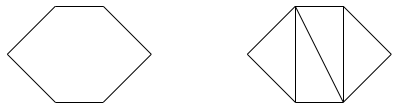
\includegraphics[width=5cm]{hex_tri_cells}
      \caption{Hexagonal cell versus triangle cells}
      \label{fig_hex_vs_tri}
    \end{figure}
  \item[Transition elements and Adaptive Mesh Refinement:] Solvers based on
    arbitrary polyhedral cells can easily handle cells with various number of
    edges. This can be particularly useful for simulations
    with Adaptive Mesh Refinement (AMR) \cite{Jessee1998,Baker2002,Wang2010a}, 
    without having to deal with the implementation of data structures to handle 
    hanging nodes \cite{Solin2008,Bangerth2007,Arnold2000}. On \Cref{fig_amr_cells}, 
    the left cell is a pentagon whereas the two cells on the right are 
    quadrilaterals. A method based on a piecewise linear discretization can
    handle locally adapted meshes without any special treatment or further
    approximation of the coupling between cells.
    \begin{figure}[H]
      \centering
      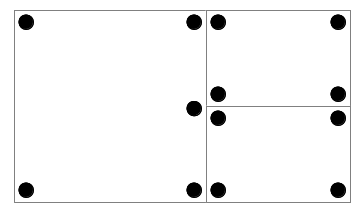
\includegraphics[width=5cm]{amr}
      \caption{AMR mesh}
      \label{fig_amr_cells}
    \end{figure}
\end{description}

%-----------------------------------------------------------
\subsection{Piecewise Linear Basis Functions on Arbitrary Polygons}
%-----------------------------------------------------------

Consider a polygonal cell with $N_V$ vertices, $(x_i,y_i)$. The polygon needs not 
to be convex. In order to describe the piecewise linear basis functions
for such a cell, we introduce a cell ``center'', denoted hereafter 
by $c=(x_c,y_c)$, with $x_c =\sum_{i=1}^{N_V} \alpha_{i} x_i$
and  $y_c = \sum_{i=1}^{N_V} \alpha_{i} y_i$. We require that
$\sum_{i=1}^{N_V} \alpha_{i} = 1$. Point $c$ is a weighted average
of the polygon's vertices. Often, one chooses $\alpha_i = 1 / N_V$.
With the introduction of the cell center, the polygon can be viewed as
$N_V$ triangular subcells, each triangle being composed of two
successive vertices and the cell center.
The $N_V$ piecewise linear basis functions are given by:
%
\begin{equation}
  b_j(\br) = t_j(\br) + \alpha_{j} t_c(\br) , \qquad j=1,\ldots,N_V ,
\end{equation}
%
where $t_j(\br)$ is the standard linear function defined on the two
triangular subcells formed by (i) vertex $j$, vertex $j-1$ and the cell center $c$,
and (ii) vertex $j$, vertex $j+1$ and the cell center $c$.
$t_j$ is equal to one at the $j^{th}$ vertex and to zero all other vertices,
as well as at the cell center.
$t_c(\br)$ is a function associated with the cell center and is equal to one 
at the cell center  and to zero at all of the polygon vertices.
%
We stress that this does not lead to a standard continuous finite element
representation within a polygon that is cut into $N_V$
triangular subcells; in such a case, the number of basis functions
would be $N_V+1$ (for the $N_V$ vertices and the cell center). In the
piecewise linear representation, the unknowns are only located at the cell 
vertices and the cell center point is only used to define the basis functions.

Put figures with PWL contour plots in a pentagon and in the degenerate pentagon.

In this
research, we focus on using PWLD to discretize the diffusion equation. The
PWLD discretization employs discontinuous finite elements and has been used to
discretize the transport equation. Using it to discretize the diffusion
equation is an important step in order to create a Diffusion Synthetic
Acceleration scheme \cite{Adams2002,Wang2010}.


%%%%%%%%%%%%%%%%%%%%%%%%%%%%%%%%%%%%%%%%%%%%%%%%%%%%%%%%%%%%%%%%%%%%%%%%%%%%%%%%%%%%%%%%%%%%%%%%%%%%
%%%%%%%%%%%%%%%%%%%%%%%%%%%%%%%%%%%%%%%%%%%%%%%%%%%%%%%%%%%%%%%%%%%%%%%%%%%%%%%%%%%%%%%%%%%%%%%%%%%%
\section{Finite Element Formulation} \label{sec:ip}
%%%%%%%%%%%%%%%%%%%%%%%%%%%%%%%%%%%%%%%%%%%%%%%%%%%%%%%%%%%%%%%%%%%%%%%%%%%%%%%%%%%%%%%%%%%%%%%%%%%%
%%%%%%%%%%%%%%%%%%%%%%%%%%%%%%%%%%%%%%%%%%%%%%%%%%%%%%%%%%%%%%%%%%%%%%%%%%%%%%%%%%%%%%%%%%%%%%%%%%%%
 
%-----------------------------------------------------------
\subsection{SIP}
%-----------------------------------------------------------

%-----------------------------------------------------------
\subsection{AMG}
%-----------------------------------------------------------

%%%%%%%%%%%%%%%%%%%%%%%%%%%%%%%%%%%%%%%%%%%%%%%%%%%%%%%%%%%%%%%%%%%%%%%%%%%%%%%%%%%%%%%%%%%%%%%%%%%%
%%%%%%%%%%%%%%%%%%%%%%%%%%%%%%%%%%%%%%%%%%%%%%%%%%%%%%%%%%%%%%%%%%%%%%%%%%%%%%%%%%%%%%%%%%%%%%%%%%%%
\section{AMR} \label{sec:amr}
%%%%%%%%%%%%%%%%%%%%%%%%%%%%%%%%%%%%%%%%%%%%%%%%%%%%%%%%%%%%%%%%%%%%%%%%%%%%%%%%%%%%%%%%%%%%%%%%%%%%
%%%%%%%%%%%%%%%%%%%%%%%%%%%%%%%%%%%%%%%%%%%%%%%%%%%%%%%%%%%%%%%%%%%%%%%%%%%%%%%%%%%%%%%%%%%%%%%%%%%%

In radiation transport and radiative transfer, lower-order spatial schemes are most commonly used. The AMR techniques employed with such schemes typically rely on gradient-based error estimates \cite{Jessee1998380}, with a few exceptions, e.g., \cite{kanschat-rad-transfer-97}, where an adjoint-based estimator is derived.
Here, we wish to obtain error estimates for high-order spatial approximations and, therefore, may not rely on simpler estimates such as the gradient of the solution. We have chosen to follow several approaches to estimate the spatial discretization error and propose three means for controlling the spatial error in $S_N$ calculations. The first technique employs two adapted AMR meshes at each adaptivity cycle: a coarse AMR mesh $\mathbb{T}_h^k$ and a fine AMR mesh $\mathbb{T}_{h/2}^k$ obtained by uniform refinement of $\mathbb{T}_h^k$; in the preceding, $k$ denotes the mesh adaptivity cycle index. Error estimates are obtained using the two solutions computed on $\mathbb{T}_{h}^k$ and $\mathbb{T}_{h/2}^k$. This approach is also discussed in \cite{demko-book1,Solin2004449}. The second error estimation technique proposed here is a simple variant of the above technique, where the coarse solution is not computed but approximated by projecting the finer solution onto the coarser mesh. The third approach presented is heuristic and monitors the inter-element jumps of the solution across elements. We discuss these three error estimates below. For goal-oriented AMR, the estimates 
described here can be re-used ``as is''; see Section~\ref{sec:go-error}.



%%%%%%%%%%%%%%%%%%%%%%%%%%%%%%%%%%%%%%%%%%%%%%%%%%%%%%%%%%%%%%%%%%%%
\subsection{Refinement Criteria} \label{sec:error4}
%%%%%%%%%%%%%%%%%%%%%%%%%%%%%%%%%%%%%%%%%%%%%%%%%%%%%%%%%%%%%%%%%%%%

The criterion for refinement is defined as follows: an element $K$ of $\mathbb{T}_h^k$ is selected for refinement if
\be
\beta _{K}^{k} \ge \alpha \, \max_{K'\in \mathbb{T}_{h}^k} \left( \beta _{K'}^{k} \right),
\label{eq:criterion}
\ee
where $\alpha$ ($0 < \alpha < 1$) is a user-defined fraction and $\beta$ stands for any of the error estimates ($\mu$, $\eta$, $\zeta$, $\widetilde \mu$, $\widetilde \eta$, and $\widetilde \zeta$)
previously defined in \eqt{eq:error-est1}, \eqt{eq:error-est2}, \eqt{eq:error-jump} or \eqt{eq:error-go}. 
The criterion of \eqt{eq:criterion} focuses the computational effort on elements with the largest errors; for
standard AMR, this tends to naturally equi-distribute the spatial error, whereas for goal-oriented approaches
this aims at reducing the computational effort for a given quantity of interest. 


 
%%%%%%%%%%%%%%%%%%%%%%%%%%%%%%%%%%%%%%%%%%%%%%%%%%%%%%%%%%%%%%%%%%%%%%%%%%%%%%%%%%%%%%%%%%%%%%%%%%%%
%%%%%%%%%%%%%%%%%%%%%%%%%%%%%%%%%%%%%%%%%%%%%%%%%%%%%%%%%%%%%%%%%%%%%%%%%%%%%%%%%%%%%%%%%%%%%%%%%%%%
\section{Results} \label{sec:results}
%%%%%%%%%%%%%%%%%%%%%%%%%%%%%%%%%%%%%%%%%%%%%%%%%%%%%%%%%%%%%%%%%%%%%%%%%%%%%%%%%%%%%%%%%%%%%%%%%%%%
%%%%%%%%%%%%%%%%%%%%%%%%%%%%%%%%%%%%%%%%%%%%%%%%%%%%%%%%%%%%%%%%%%%%%%%%%%%%%%%%%%%%%%%%%%%%%%%%%%%%

We present five examples to validate our approach.  

%%%%%%%%%%%%%%%%%%%%%%%%%%%%%%%%%%%%%%%%%%%%%%%%%%%%%%%%%%%%%%%%%%%%%%%%%%%%%%%%%%%%%%%%%%%%%%%%%%%%
\subsection{Example 1} \label{sec:ex1}
%%%%%%%%%%%%%%%%%%%%%%%%%%%%%%%%%%%%%%%%%%%%%%%%%%%%%%%%%%%%%%%%%%%%%%%%%%%%%%%%%%%%%%%%%%%%%%%%%%%%


%%%%%%%%%%%%%%%%%%%%%%%%%%%%%%%%%%%%%%%%%%%%%%%%%%%%%%%%%%%%%%%%%%%%%%%%%%%%%%%%%%%%%%%%%%%%%%%%%%%%
%%%%%%%%%%%%%%%%%%%%%%%%%%%%%%%%%%%%%%%%%%%%%%%%%%%%%%%%%%%%%%%%%%%%%%%%%%%%%%%%%%%%%%%%%%%%%%%%%%%%
%%%%%%%%%%%%%%%%%%%%%%%%%%%%%%%%%%%%%%%%%%%%%%%%%%%%%%%%%%%%%%%%%%%%%%%%%%%%%%%%%%%%%%%%%%%%%%%%%%%%



%%%%%%%%%%%%%%%%%%%%%%%%%%%%%%%%%%%%%%%%%%%%%%%%%%%%%%%%%%%%%%%%%%%%%%%%%%%%%%%%%%%%%%%%%%%%%%%%%%%%
%%%%%%%%%%%%%%%%%%%%%%%%%%%%%%%%%%%%%%%%%%%%%%%%%%%%%%%%%%%%%%%%%%%%%%%%%%%%%%%%%%%%%%%%%%%%%%%%%%%%
%%%%%%%%%%%%%%%%%%%%%%%%%%%%%%%%%%%%%%%%%%%%%%%%%%%%%%%%%%%%%%%%%%%%%%%%%%%%%%%%%%%%%%%%%%%%%%%%%%%%
\pagebreak

\begin{figure}[h]
\begin{center}
\includegraphics[scale=1.]{two-mesh.eps}
\end{center}
\caption{Schematics of the two-mesh AMR approach.}
\label{fig:2-mesh-schematics}
\end{figure}

%%%%%%%%%%%%%%%%%%%%%%%%%%%%%%%%%%%%%%%%%%%%%%%%%%%%%%%%%%%%%%%%%%%%%%%%%%%%%%%%%%%%%%%%%%%%%%%%%%%%
\pagebreak

\begin{figure}[h]
\begin{center}
\includegraphics[scale=0.4]{ref-rules2.eps}
\end{center}
\caption{Refinement rule: the original triangle is bisected into 4 smaller triangles; 
local numbering rules are defined; a tree structure is employed to obtain the refinement level depth.}
\label{fig:triangle-ref-rule}
\end{figure}

%%%%%%%%%%%%%%%%%%%%%%%%%%%%%%%%%%%%%%%%%%%%%%%%%%%%%%%%%%%%%%%%%%%%%%%%%%%%%%%%%%%%%%%%%%%%%%%%%%%%
\pagebreak

\begin{figure}[!hbtp]
\centering
\subfigure[0-level refinement difference]{
\includegraphics[scale=0.45]{edge-coupling-0}
\label{fig:sub_edge0}
}
\subfigure[1-level refinement difference]{
\includegraphics[scale=0.45]{edge-coupling-1}
\label{fig:sub_edge1}
}
\subfigure[1-level refinement difference]{
\includegraphics[scale=0.45]{edge-coupling-1b}
\label{fig:sub_edge1b}
}
\caption{Cases of edge coupling.}
\label{fig:edge_coupling_fig}
\end{figure}


%%%%%%%%%%%%%%%%%%%%%%%%%%%%%%%%%%%%%%%%%%%%%%%%%%%%%%%%%%%%%%%%%%%%%%%%%%%%%%%%%%%%%%%%%%%%%%%%%%%%

\pagebreak

\begin{figure}[h]
\begin{minipage}[b]{1.\linewidth}
%
\begin{center}
\subfigure[Two-mesh AMR]
{
\includegraphics[width=3.5cm]{mesh-TB-est-2mesh-c14-p-1.ps}
\includegraphics[width=3.5cm]{mesh-TB-est-2mesh-c14-p-2.ps}
\includegraphics[width=3.75cm]{mesh-TB-est-2mesh-c14-p-3.ps}
\includegraphics[width=4.35cm]{mesh-TB-est-2mesh-c14-p-4.ps} 
}
\end{center}
\end{minipage}
%
\begin{minipage}[b]{1.\linewidth}
\begin{center}
\subfigure[Jump-based AMR ]
{
\includegraphics[scale=0.17]{mesh-TB-jump-c14-p1.ps}
\includegraphics[scale=0.17]{mesh-TB-jump-c14-p2.ps}
\includegraphics[scale=0.17]{mesh-TB-jump-c14-p3.ps}
\includegraphics[scale=0.17]{mesh-TB-jump-c14-p4.ps}
}
\end{center}
\end{minipage}
\caption{Example 3: Adapted meshes. From left to right, $p=1,\,2,\,3,\,4$}
\label{fig:ex3-meshes}
\end{figure}


%%%%%%%%%%%%%%%%%%%%%%%%%%%%%%%%%%%%%%%%%%%%%%%%%%%%%%%%%%%%%%%%%%%%%%%%%%%%%%%%%%%%%%%%%%%%%%%%%%%%
%%%%%%%%%%%%%%%%%%%%%%%%%%%%%%%%%%%%%%%%%%%%%%%%%%%%%%%%%%%%%%%%%%%%%%%%%%%%%%%%%%%%%%%%%%%%%%%%%%%%
%%%%%%%%%%%%%%%%%%%%%%%%%%%%%%%%%%%%%%%%%%%%%%%%%%%%%%%%%%%%%%%%%%%%%%%%%%%%%%%%%%%%%%%%%%%%%%%%%%%%
%%%%%%%%%%%%%%%%%%%%%%%%%%%%%%%%%%%%%%%%%%%%%%%%%%%%%%%%%%%%%%%%%%%%%%%%%%%%%%%%%%%%%%%%%%%%%%%%%%%%
%\include{bibli.bib}
%\bibliographystyle{unsrt}
%\bibliography{bibli}

\pagebreak


\begin{thebibliography}{100}


\end{thebibliography}



%%%%%%%%%%%%%%%%%%%%%%%%%%%%%%%%%%%%%%%%%%%%%%%%%%%%%%%%%%%%%%%%%%%%%%%%%%%%%%%%%%%%%%%%%%%%%%%%%%%%
%%%%%%%%%%%%%%%%%%%%%%%%%%%%%%%%%%%%%%%%%%%%%%%%%%%%%%%%%%%%%%%%%%%%%%%%%%%%%%%%%%%%%%%%%%%%%%%%%%%%
\end{document}
%%%%%%%%%%%%%%%%%%%%%%%%%%%%%%%%%%%%%%%%%%%%%%%%%%%%%%%%%%%%%%%%%%%%%%%%%%%%%%%%%%%%%%%%%%%%%%%%%%%%
%%%%%%%%%%%%%%%%%%%%%%%%%%%%%%%%%%%%%%%%%%%%%%%%%%%%%%%%%%%%%%%%%%%%%%%%%%%%%%%%%%%%%%%%%%%%%%%%%%%%
